\chapter{Preliminares}

En este capítulo vamos a presentar las herramientas básicas para llevar a cabo nuestra teoría. Empezaremos recordando conceptos básicos de probabilidad, presentaremos algunos resultados relacionados con las matrices y finalmente introduciremos técnicas que se utilizan en la estadística y en la computación.

\section{Conceptos básicos de probabilidad}
Comenzamos presentado los elementos necesarios para considerar una probabilidad:
\begin{definition}
    Sea $\Omega$ un conjunto arbitrario, diremos que una familia no vacía de subconjuntos de $\Omega$, $\mathcal{A}\subseteq\mathcal{P}(\Omega)$, es una $\sigma$-álgebra si:
    \begin{itemize}
        \item Es cerrada para complementarios: $\forall A\in\mathcal{A},\, \Omega\setminus A\in\mathcal{A}.$
        \item Es cerrada para uniones numerables: si $A_{n}\in\mathcal{A}, \,\forall n\in\mathbb{N}  \implies \displaystyle\bigcup_{n\in\mathbb{N}}A_n\in\mathcal{A}.$
    \end{itemize}
\end{definition}

A la dupla $(\Omega,\mathcal{A})$ se le conoce como espacio medible.
\begin{definition}
    Sea $(\Omega,\mathcal{A})$ un espacio medible, $P:\mathcal{A}\longrightarrow [0,1]$ es una probabilidad si:
    \begin{itemize}
        \item $P(A)\geq 0, \, \forall A\in\mathcal{A}.$
        \item $P(\Omega)=1.$
        \item Dada una secuencia $\{A_{n}\}_{n\in\mathbb{N}}\subseteq\mathcal{A}$ con $A_i\centernot\cap A_j$, $i\neq j$ entonces:
        \[P\left(\bigcup_{n\in\mathbb{N}}A_n\right)=\sum_{n\in\mathbb{N}}P(A_n)\]
    \end{itemize}
\end{definition}
A la terna $(\Omega,\mathcal{A},P)$ se le conoce como espacio probabilístico.
\begin{definition}
    Sea $(\Omega,\mathcal{A},P)$ un espacio probabilístico y $A\in\mathcal{A}$ con $P(A)>0$. Sea $B\in\mathcal{A}$, se define la probabilidad condicionada de $B$ dado $A$ como:
    \[P(B|A)=\dfrac{P(B\cap A)}{P(A)}\]
\end{definition}
Relacionado con esta definición presentamos el siguiente teorema que nos será útil:
\begin{theorem}[Teorema de probabilidad total]
    Sea $(\Omega,\mathcal{A},P)$ un espacio probabilístico y $\{A_{n}\}_{n\in\mathbb{N}}\subseteq\mathcal{A}$ una partición de $\Omega$ con $P(A_n)>0, \,\forall n \in \mathbb{N}$. Sea $B\in\mathcal{A}$, entonces:
    \[P(B)=\sum_{n\in\mathbb{N}}P(A_n)P(B|A_n)\]
\end{theorem}
\begin{proofs*}
    Por ser $\{A_n\}$ una partición de $\Omega$, aplicando la definición de probabilidad condicionada:
    \[P(B)=P\left(\bigcup_{n\in\mathbb{N}}B\cap A_n\right)=\sum_{n\in\mathbb{N}}P(B\cap A_n)
        =\sum_{n\in\mathbb{N}}P(A_n)P(B|A_n)\]\qed
\end{proofs*}

\begin{definition}
 Sea $(\Omega,\mathcal{A},P)$ un espacio probabilístico y $(\Omega',\mathcal{A}')$ un espacio medible. Una función $X:(\Omega,\mathcal{A},P)\longrightarrow(\Omega',\mathcal{A}')$ es una variable aleatoria si:
 \[X^{-1}(B)\in\mathcal{A}, \quad \forall B\in\mathcal{A}'\]
\end{definition}

\section{Resultados sobre matrices}
Para el estudio de las cadenas de Markov, necesitamos de antemano algunos resultados sobre matrices. Por comodidad, usaremos a lo largo de este trabajo la notación fila para representar los vectores. Los contenidos de esta sección se basa principalmente en \cite{Salinelli}.

\begin{definition}
    Sea una matriz $A=[a_{ij}]$, diremos que $A$ es:
    \begin{itemize}
        \item \textbf{no negativa} si $a_{ij}\geq 0,\, \forall i,j$.
        \item \textbf{positiva} si $a_{ij}\geq 0,\, \forall i,j$ y existe $a_{ij}>0$ para al menos un par de índices $i,\,j$.
        \item \textbf{estrictamente positiva} si $a_{ij}> 0,\, \forall i,j$.
    \end{itemize}
\end{definition}

\begin{definition}
    Sea $A=[a_{ij}]$ una matriz cuadrada de dimensión $N$, diremos que $A$ es una \textbf{matriz estocástica} si:
    \[
    \begin{aligned}
    a_{ij}\in[0,1],\quad \forall i,j \in \{1,...,N\},\\
    \sum_{j=1}^N a_{ij}=1, \quad \forall i\in\{1,...,N\}.
    \end{aligned}
    \]
\end{definition}

Una forma de caracterizar a las matrices estocásticas es mediante la siguiente proposición:

\begin{proposition}\label{propiedadMatrizEstocástica}
Sea $A$ una matriz cuadrada positiva de dimensión $N\times N$:
\begin{enumerate}
    \item $A$ es estocástica si y solo si $1$ es un valor propio de $A^T$ con vector propio $\mathbf{1}=\begin{pmatrix}1 & 1 & \dots & 1\end{pmatrix}$.
    \item si $A$ es estocástica, entonces para todo valor propio $\lambda$, se cumple que  $\left|\lambda\right|\leq1.$
\end{enumerate}
\end{proposition}

\begin{proofs*}
\
\begin{enumerate}
    \item Es suficiente con observar que la condición de estocasticidad para una matriz positiva $A$ es equivalente a que $\mathbf{1}\cdot A^T=\mathbf{1}$.
    \item Sea $v=(v_1,\dots,v_N)$ un vector propio asociado a $\lambda$ (a izquierda pues estamos usando la notación fila), por ser $A$ positiva y estocástica, se verifica:
    \[
    \begin{aligned}
        \left|\lambda\right|\sum_{j=1}^N\left| v_j\right|&=\sum_{j=1}^N\left|\lambda v_j\right|= \sum_{j=1}^N\left|(vA)_j \right|  =\sum_{j=1}^N\left|\sum_{i=1}^N a_{ij}v_i\right|\\
        &\leq\sum_{j=1}^N\sum_{i=1}^N a_{ij}\left|v_i\right|=\sum_{i=1}^N\left( \sum_{j=1}^N a_{ij} \right) \left|v_i\right|=\sum_{i=1}^N\left|v_i\right|    
    \end{aligned}
    \]
    Puesto que $\displaystyle\sum_{r=1}^N\left|v_r\right|>0$, tenemos que $\left|\lambda\right|\leq1$.    \qed
\end{enumerate}
\end{proofs*}

\begin{remark*}\label{productoEstocásticos}
De la primera afirmación de la proposición \ref{propiedadMatrizEstocástica}, podemos ver que el producto de matrices estocásticas sigue siendo estocástica. En efecto, si $A$ y $B$ son dos matrices estocásticas entonces $\mathbf{1}\cdot\left(AB\right)^T=\mathbf{1}\cdot B^T\cdot A^T=\mathbf{1}\cdot A^T=\mathbf{1}$.
\end{remark*}

Presentamos a continuación la definición de un grafo dirigido y el grafo de una matriz no negativa:
\begin{definition}
    Un grafo dirigido $G$ es un par $(V,L)$ donde $V=\{v_1,\dots,v_n\}$ es un conjunto finito de elementos llamados \textbf{nodos} (o \textbf{vértices}) y $L=\{l_1,\dots,l_m\}\subseteq V\times V$ es un conjunto de pares ordenados de dichos nodos llamados \textbf{arcos} (o \textbf{aristas}).
\end{definition}

\begin{definition}
    Sea $G=(V,L)$ un grafo dirigido, un \textbf{camino dirigido} $C$ desde $v_{i_0}$ a $v_{i_p}$ es una secuencia de nodos $C=\{v_{i_0},v_{i_1}, \dots, v_{i_p}\}$ tal que $v_{i_k}\in V$ para todo $k=0,\dots,p$ y $(v_{i_{k-1}}, v_{i_k})\in L$ para todo $k=1,\dots,p$. 
\end{definition}

\begin{definition}
    Sea $G=(V,L)$ un grafo dirigido, diremos que:
    \begin{itemize}
        \item un nodo $v_i\in V$ está \textbf{conectado} con un nodo $v_j\in V$ si existe un camino dirigido de $v_i$ a $v_j$.
        \item un nodo $v_i\in V$ está \textbf{fuertemente conectado} con un nodo $v_j\in V$ si ambos están conectados.
    \end{itemize}
    Un grafo dirigido es \textbf{fuertemente conectado} si sólo tiene un nodo o todos sus nodos están fuertemente conectados entre ellos.
\end{definition}

\begin{definition}
    Sea $A$ una matriz cuadrada no negativa de dimensión $N$, el grafo dirigido asociado a $A$ es de la forma $G_A=(V_A,L_A)$ donde:
    \[V_A=\{1,\dots,N\}\] 
    \[L_A=\{(i,j)\in V_A\times V_A \,|\, a_{ij}>0\}\]
\end{definition}

\begin{exampleth}
    Dada la matriz:
    \[A=\begin{pmatrix}
        2 & 0 & 1 & 6 \\
        0 & 4 & 2 & 3 \\
        1 & 5 & 0 & 0 \\
        7 & 3 & 1 & 1 
    \end{pmatrix}\]
    Podemos representar su grafo asociado:
    \begin{center}
        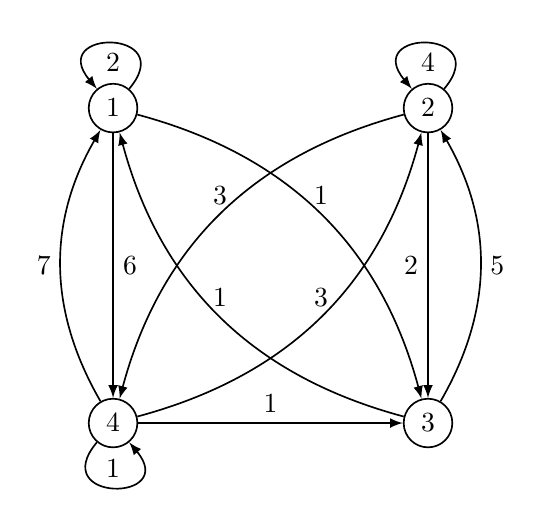
\begin{tikzpicture}[-latex ,auto , node distance =4 cm ,semithick,
        main/.style = {draw, circle}] 
            \node[main] (1) {$1$}; 
            \node[main] (2) [right of=1] {$2$};
            \node[main] (3) [below of=2] {$3$};
            \node[main] (4) [below of=1] {$4$};
            
            \path (1) edge[distance=1cm, out=50, in=130] node {2} (1);
            \draw (1) edge [bend left] node [above] {1} (3);
            \draw (1) edge node {6} (4);

            \path (2) edge[distance=1cm, out=50, in=130] node {4} (2);
            \draw (2) edge node[left] {2} (3);
            \draw (2) edge[bend right] node [above] {3} (4);

            \path (3) edge[bend left] node [above] {1} (1);
            \path (3) edge[bend right] node[right] {5} (2); 

            \path (4) edge[bend left] node {7} (1); 
            \path (4) edge[bend right] node [above] {3} (2);
            \path (4) edge node {1} (3);
            \path (4) edge[distance=1cm, out=230, in=310] node {1} (4);
            
        \end{tikzpicture}
    \end{center}
    El grafo de esta matriz es fuertemente conectado pues desde cualquier nodo podemos encontrar un camino dirigido a los otros nodos, incluido a sí mismo.
\end{exampleth}